\documentclass[10pt, final]{article}

\usepackage{algorithm2e}
\usepackage{amsmath}
\usepackage{cite}
\usepackage{graphicx}
\usepackage{fullpage}
\usepackage{hyperref}
\usepackage{url}

% Line break with additional spacing. Default is .75 line-height extra spacing
% Extra space is put in to allow line breaks immediately after \item
\newcommand{\br}[1][.75]{\ \\[#1\baselineskip]}

\parindent 0pt

\begin{document}

\begin{center}
\LARGE{\textbf{Tag Recommendations in StackOverflow}}\\
\Large{\textbf{CS 224W Project Milestone}}\\
\Large{Logan Short, Christopher Wong, David Zeng}
\end{center}

\section{Introduction}

In many community-based information web sites, such as StackOverflow, users contribute content in the form of questions and answers, allowing others to learn through the collaboration and contributions of the community. These web sites often rely upon tags as metadata that assists in the indexing, categorization, and search for particular content with just a few key words. Almost always, users are given the responsibility to choose tags which identify their own content. Human error suggests, then, that this content is not always well-tagged. As such, tag recommendation systems are helpful to guide users into labeling their content with the most appropriate tags.\br
Our project addresses the problem of recommending tags in community-based information web sites such as StackOverflow by improving on existing implementations through the use of the underlying network structure of the web site. We begin by reviewing and critiquing various research papers related to our topic in Section $2$. Then, in Section $3$, we explain our methods for collecting and parsing our data from the StackOverflow data dump. In Section $4$, we summarize our initial findings and statistics about our data set, and discuss the possible implications this may have on our eventual final results. Finally, in Sections $5$ and $6$, we outline the remaining work for this project.


\section{Related Work}

Before critiquing existing implementations of tag recommendation systems, we found abundant relevant information regarding the growth and properties of groups and communities in large social networks. In \cite{2}, McAuley and Leskovec propose an algorithm to automatically discover social circles by analyzing the similarities among user profiles in data drawn from the social networking sites Facebook, Google+, and Twitter. Using the idea that nodes are well connected within a circle, the algorithm finds the best parameters to determine which edges should exist in an ego network. In \cite{3}, Backstrom et al. analyze the evolution of communities in social networks over time. The authors use a decision tree model to classify communities as fast- or slow-growing and show that connectedness of the community within and to those outside of the community plays a huge role in growth rate.\br
In \cite{1}, Xia et al. propose an automatic tag recommendation algorithm \textit{TagCombine}. There are three components of \textit{TagCombine}, each of which tries to assign the best tags to untagged objects: (1) multi-label ranking component, which predicts tags using a multi-label learning algorithm, (2) similarity based ranking component, which uses similar objects to recommend tags, and (3) tag-term based ranking component, which analyzes the historical affinity of tags to certain words in order to suggest tags. The recommendation algorithm methodically computes various weighted sums of the three components to attempt to find the best overall model. A $recall@k$ score is then calculated for each prediction model from stratified $10$-fold cross validation. (The $recall@k$ metric is discussed more in Section $4$.) \textit{TagCombine} does significantly better than all other cited models.\br
In \cite{5}, Wang et al. propose a tag recommendation system dubbed \textit{EnTagRec}. The proposed \textit{EnTagRec} computes tag probability scores using two separate methods, Bayesian Inference and Frequentist Inference, and then takes a weighted sum of the probability scores. Bayesian Inference relies on a post's textual data to compute the probability that a given tag is associated with the post. \textit{EnTagRec} formulates posts into a bag-of-words model and then trains a Labeled Latent Dirichlet Allocation model which is used to compute tag probability scores for a post. The Frequentist Inference approach infers a set of tags after some preprocessing of a post. Once this set is computed, \textit{EnTagRec} applies spreading activation to a tag network constructed by examining the co-occurrence rate of tags on the site. Experimental results show that \textit{EnTagRec} performs significantly better than \textit{TagCombine} from \cite{1} on Stack Overflow, Ask Ubuntu, and Ask Different datasets, but yields only comparable results on Freecode datasets.\br
In \cite{1}, Xia et al. propose a recommendation system that relates the textual features of posts to tags with reasonably good results. However, one weakeness of \textit{TagCombine} is that it fails to look at the network structure of software information sites. Posts on sites like Stack Overflow are ultimately connected to each other through an underlying network structure where users and tags that appear on multiple posts represent connections between said posts. In fact, tags exist in order to group similar posts and create an organized structure that allows for more convenient and logical browsing of posts. Thus, it makes sense that knowledge of the network's structure could be used to enhance a tag recommendation system. In \cite{5}, Wang et al. provide evidence that such an approach could yield significant improvement in tag recommendation results. In \cite{5}, the basic \textit{TagCombine} model proposed in \cite{1} is enhanced into a model that uses not only textual analysis of posts, but also network analysis of the tags themselves. Although results improved, the use of network structure is very limited, and further incorporation of network structure could potentially lead to more accurate tag recommendations.\br
One weakness in both \cite{1} and \cite{5} is that they both only address tag recommendations during question creation time. That is, tag recommendations need to be made with just the text from the initial post. Discussion generated over time by the post is not factored into the features for the tag recommendation system. However, tagging a post is not an action limited to post creation time. Users may add additional tags to posts later on based on the discussion. In the context of a social network, this is similar to the notion of users joining new communities: posts can acquire new tags over time. This train of thought brings us back to the discussion of clustering of nodes in networks. In \cite{2}, McAuley and Leskovec discuss a method for automatically detecting ``circles'' in networks of users based on similarities in user profiles. A natural extension of this method would be to detect posts associated with common tags based on the similarities in features of the posts or to find circles of tags or users that could allow for accurate detection of possible associated tags using a given tag. Both situations are realistic for clustering tags, users, or posts on software information sites.


\section{Data Collection}

StackOverflow is a member of the Stack Exchange network, and all user content contributed on this network is cc-by-sa 3.0 licensed. Our data set is the September 26, 2014 snapshot for StackOverflow, downloaded from the Stack Exchange data dump (see \cite{6}). The raw data set contains approximately 20 gigabytes (GB) of compressed XML files corresponding to Badges, Comments, PostHistory, PostLinks, Posts, Tags, Users, and Votes.\br
Uncompressing the data files revealed there to be 3,473,094 users, 21,736,594 posts, 32,506,636 comments, and 38,205 tags in our data dump. As the total size of the dump approached 100 GB in total, we immediately made decisions regarding how to strip down the data set to make running computations more manageable. To start, we converted all of the files to CSV files, thereby avoiding the verbosity of XML. Perhaps more importantly, we made intuitive decisions on various attributes that could be dropped during our filter. For example, the data dump provides the complete text for the ``About Me'' section of every user's profile page, but we found it unlikely that this would provide any assistance for our tag recommendations.\br
For one final data management optimization, we further split up our per-category CSV files into various partitions such as \texttt{posts-metadata.csv} and \texttt{posts-body.csv}. This allowed some of our initial individual algorithms to run faster since they received as input only the data that was necessary. For example, our network analysis of StackOverflow generally only required the posts' metadata (ex. creationTime, viewCount, userID), whereas the lexical modelling of the posts themselves clearly required the posts' lengthy text bodies.

\section{Initial Findings}

The initial steps of our project can be broken down into two areas. In Section $4.1$, we discuss our implementation of the components of \textit{TagCombine} as described in \cite{1}. In Section $4.2$, we analyze the network and community structure of the StackOverflow network, giving us motivation for the next steps in our project to improve upon tag recommendation systems.

\subsection{\textit{TagCombine} Components}

To start, using the procedures described in \cite{1}, we implemented the three major components of the \textit{TagCombine} algorithm to establish a baseline for the performance of our tag recommendation system. By reproducing a working implementation of \textit{TagCombine}, we can analyze the effect of our improvements on tag recommendation accuracy.\br
As alluded to earlier, \cite{1} introduces the concept of the $recall@k$ metric for measuring the success of a tag recommendation model, where $k$ is a tunable parameter that determines how many tags the model recommends for each object. Intuitively, over $n$ objects, the $recall@k$ metric measures the average success rate in predicting correct tags for each object, where a ``correct'' tag is simply a tag that has been used to label that particular object by an actual user. Let $R_i$ be the set of tags recommended for object $i$ (so, $|R_i| = k$), and let $T_i$ be the actual set of tags used to label object $i$. Then, the formula for $recall@k$ is:

\[recall@k = \frac{1}{n}\sum\limits_{i=1}^{n}\frac{|R_i \cap T_i|}{|T_i|}.\]

For the purposes of evaluating our initial implementation in a timely manner, we chose to look at only the first $50,000$ questions posted on StackOverflow, with creation dates ranging from July 2008 to December 2008. We also preprocessed the text of each post, using the \texttt{snowballstemmer-1.2.0} Python package to stem word tokens. To emulate \cite{1}, we also removed any terms from our consideration set that did not appear at least $20$ times. Finally, we considered only the tags that appeared more than $50$ times among the first batch of questions, since less-common tags would not likely be recommended to a user. For reasons we will discuss, instead of methodically checking all combinations of different weights for the three components, we evaluated each component of our implementation as standalone using $10$-fold cross validation:

\begin{center}\begin{tabular}{c||c|c}
& $recall@5$ & $recall@10$\\ \hline\hline
Multilabel Classifier & 0.556 & 0.641\\ \hline
Similarity Ranking & 0.478 & 0.581\\ \hline
Tag Term Affinity & 0.254 & 0.346\\ \hline\hline
\cite{1} Original \textit{TagCombine} & 0.596 & 0.724\\
\end{tabular}\end{center}

One can clearly see that the Multilabel Classifier (bag of words) performs the best, followed by the Similarity Ranking, and then the Tag Term Affinity scores. Furthermore, no single component does better than the aggregate \textit{TagCombine} algorithm, which is to be expected. We note that, due to the way in which weights are assigned to components in the \textit{TagCombine} algorithm, the aggregate model will perform better than the individual components \cite{1}.\br
Analyzing the components individually allows us to view a few properties of each. For example, below are two scatterplots of the post text length against the $recall@5$ and $recall@10$ scores for the Similarity component.

\begin{center}
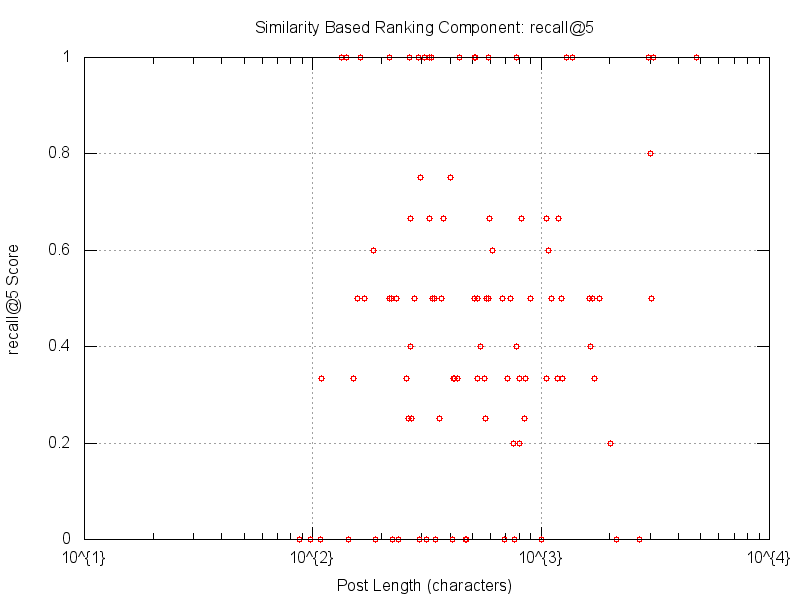
\includegraphics[width=3.2in]{sim-50000-recall5.png}
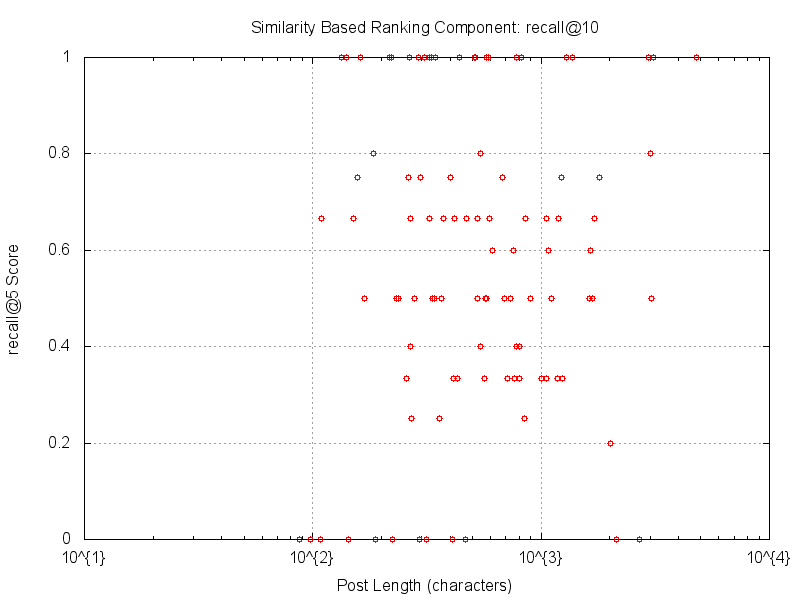
\includegraphics[width=3.2in]{sim-50000-recall10.png}
\end{center}

There does not seem to be any correlation between the text length and the $recall@k$ scores, which is good, as similarity measures can often suffer from bias towards longer samples of data.\br
Furthermore, by isolating our multilabel classifier and running it standalone, we were able to focus on which features gave us the best $recall@k$ scores, as will be discussed more in Section $4.2$. Instead, if we had run the \textit{TagCombine} aggregate iteration algorithm, it is likely that more of our attention and analysis would have been focused on picking correct weights. Still, the fact that \textit{TagCombine} was able to effectively combine several weaker tag recommenders into one stronger recommender suggests that the process could be further improved through the inclusion of recommendation systems that make up for the flaws of \textit{TagCombine}.


\subsection{Network Community Analysis}

We would like to address the weaknesses of the \textit{TagCombine} method, as described in Section 2, by utilizing features from the network structure of StackOverflow. Given the way tags organize posts on StackOverflow, it is likely that looking at the community structure of StackOverflow will give us more information on how to select the best tags. Our initial analysis of the StackOverflow network focused on the users. We ran a Bernoulli Naive Bayes Multilabel Classifier on the first $10,000$ questions posted on StackOverflow that predicted tags using feature vectors constructed by looking at which users had interacted on posts with known tags. Evaluating this method using $recall@k$ gave surprisingly good results with a $0.723$ $recall@5$ value and a $0.734$ $recall@10$ value. This is a strong indication that the interaction of users with each other and with tags could be used to strengthen the accuracy of a tag recommendation system.\br
We experimented with the following StackOverflow network. The users of StackOverflow are represented as nodes of our network. Two users $u$ and $v$ are linked with an edge if $u$ answers a question posted by $v$ such that the answer reaches a predefined threshold in positive rating. We then used the Snap implementation of the Clauset-Newman-Moore community detection algorithm to cluster the users into communities. With these communities, we attempted to recommend tags in the following manner. Given a new question, consider the user posting the question and the community the user belongs in. For each tag $t$, compute $w_t = \frac{c_t}{s_t}$, where $c_t$ denotes the number of times a question posted by a community member used the tag $t$, and $s_t$ denotes the total number of times tag $t$ is used in all of StackOverflow. The tags with the highest values of $w_t$ are selected as tag recommendations. Essentially, members of the community are voting for which tags best represent the community, with votes inversely weighted by their overall popularity in StackOverflow. With this method, we achieved a $recall@5$ value of $0.220$ and a $recall@10$ value of $0.308$. Of course, one would not expect these $recall@k$ values to be spectacular, since the tag suggestions are fixed for a given community. However, we see that even with such a simple method, we were indeed able to find some relationship between how users structure themselves into communities based on their question and answer activity, and what tags these users often use. This provides a starting point for additional experimentations, which we will describe in Section $5$.\br
Our main improvement to the tag recommendation model \textit{TagCombine} will be the addition of a \textbf{fourth} component to the weighted algorithm, one that is focused on utilizing the community structure of the StackOverflow network. We hope our final algorithm, which we will name \textit{ComTagCombine}, will work in the following manner. Adding on to the equation given in \cite{1}, for all of the tags $t$ with respect to some post $p$, the \textit{ComTagCombine} score can be given by
\begin{align*}
ComTagCombine_p(t) =\ &\alpha \times MultiLabel_p(t) + \beta \times SimRank_p(t) +\\
&\gamma \times TagTerm_p(t) + \delta \times Community_p(t)
\end{align*}
where $\alpha,\beta,\gamma,\delta \in [0,1]$ represent the different weights of the components. Here, we have added the term of $\delta \times Community_p(t)$ to represent our new fourth component that uses the underlying network structure. To handle this fourth component, here is the pseudocode for \textit{ComTagCombine}:\br
\begin{algorithm}[H]
  \textbf{Outputs: }$\alpha,\beta,\gamma,\delta$\\
  $\alpha=0,\beta=0,\gamma=0,\delta=0$\;
  \For{\textbf{all }posts $p$}{
    \For{\textbf{all }tags $t \in TAGS$}{
      Compute \textit{MultiLabel}$_p(t)$, \textit{SimRank}$_p(t)$, \textit{TagTerm}$_p(t)$, and \textit{Community$_p(t)$}\;
    }
  }
  \For{\textbf{all }$\alpha$ from $0$ to $1$, every time increment by $0.1$}{
    \For{\textbf{all }$\beta$ from $0$ to $1$, every time increment by $0.1$}{
      \For{\textbf{all }$\gamma$ from $0$ to $1$, every time increment by $0.1$}{
        \For{\textbf{all }$\delta$ from $0$ to $1$, every time increment by $0.1$}{
          Compute \textit{ComTagCombine}$_p(t)$ for all tags $t$ on posts $p$\;
          Evaluate effectiveness of $(\alpha,\beta,\gamma,\delta)$ from $recall@k$ scores\;
        }
      }
    }
  }
  \Return Best $(\alpha,\beta,\gamma,\delta)$\;
\end{algorithm}\br
Of course, to realize this new algorithm, we will need to come up with a quantifiable way to judge the \textit{Community} score of some tag $t$ with respect to post $p$.


\section{Remaining Work}

Our latter half of the project will focus on experimentation to find the best network features to use for the \textit{Community} component of our \textit{ComTagCombine} algorithm. The first thing we would like to experiment with is different algorithms for partitioning our graph into communities, such as spectral clustering, as well as the other methods briefly mentioned in lecture: METIS, Graclus, Cluto, and clique percolation. We would also like to experiment with other network structures of StackOverflow. For example, we can instead use questions themselves as nodes, and link two questions if the same users commented or answered these questions. This essentially gives us another measure of similarity between two posts, one that is based on interactions by shared users. Using a similar method as described in Section 4.2, we can find tags that best represent each community, and match new questions to communities based on a combination of the user creating the question and the text of the question itself. Lastly, we can improve on the network structure we experimented with in Section 4.2. One extension would be to add weights to edges based on a certain property we would like to focus on; given our current findings, one property that seems promising would be to give more weights to edges that represent connections between more expert users, or, those with higher ratings. Building on top of our reasoning that clustering by users will yield positive improvement, it seems likely that expert StackOverflow users will be more reliable for predictions and tag recommendations than a user that just recently joined the community.\br
On the data side, one option that stands out would be to condense the tag space of our data set by collapsing similar tags. For example, ``zombie'' and ``zombies'' both describe zombie processes in Unix, while ``xmlparser'', ``xml-parser'', and ``xmlparsing'' all describe the same thing \cite{1}. This would remove any unnecessary damage to our $recall@k$ scores due to tag synonyms, since a generated suggestion of ``xmlparser'' should be recorded as a match of ``xml-parser''.

\section{Stretch Goals}

If there still remains time, one of our stretch goals would be to further explore one of the last points made in Section $2$: tagging a post is not an action limited to post creation time. While this has already been covered simply by the fact that we are using user interaction and collaboration -- events that happen after post creation -- to assist tag recommendations, we have so far only modeled the network based on one snapshot in time. Since we have access to the entire log of post edit history, it would be interesting to see how our tag recommendations and $recall@k$ scores would change over time given snapshots in which more or less users had contributed to certain posts. Any insights or trends would provide commentary on the effectiveness of future dynamic tag recommendations systems that constantly restructure their models along with the network itself.\br
On one final note, although \textit{EnTagRec} produced better results, we chose to use \textit{TagCombine} as a baseline for measuring our improvements to tag recommendation. There were several reasons for this decision. First, \textit{TagCombine} uses a generally simpler algorithm which made it easier to accurately reproduce. In addition, \textit{EnTagRec} incorporates some degree of network structure while assessing the accuracy of its tag recommendations. Thus, using \textit{TagCombine} as a baseline allows us to more clearly demonstrate the improvement caused by incorporating network structure. Finally, since we plan to use different network analysis methods from the simple ones implemented in \textit{EnTagRec}, it is likely that our improvements would cause a similar improvement on the accuracy of \textit{EnTagRec}. If there is time, we will implement \textit{EnTagRec} and improve upon it, much like what we plan to do for \textit{TagCombine}.



\begin{thebibliography}{1}
\bibitem{1} X. Xia, D. Lo, X. Wang, B. Zhou. Tag Recommendation in Software Information Sites. MSR, 2013.
\bibitem{2} J. McAuley, J. Leskovec. Discovering Social Circles In Ego Networks. ACM TKDD, 2014.
\bibitem{3} L. Backstrom, D. Huttenlocher, J. Kleinberg, X. Lan. Group Formation in Large Social Networks: Membership, Growth, and Evolution. KDD, 2006.
\bibitem{4} J. Leskovec, K. Lang, A. Dasgupta, M. Mahoney. Statistical Properties of Community Structure in Large Social and Information Networks. WWW, 2008.
\bibitem{5} S. Wang, D. Lo, B. Vasilescu, A. Serebrenik. EnTagRec: An Enhanced Tag Recommendation System for Software Information Sites. ICSME, 2014.
\bibitem{6} Stack Exchange Data Dump (September 26, 2014). Retrieved 2 November 2014. https://archive.org/details/stackexchange.
\end{thebibliography}

\end{document}